\documentclass{article}
\usepackage{enumerate}
\usepackage{amsmath}
\usepackage{amssymb}
\usepackage{graphicx}
\usepackage{subfigure}
\usepackage{geometry}
\usepackage{color}
\usepackage{bm}
\usepackage{indentfirst}
\usepackage{float}
\usepackage{booktabs}

\begin{document}

\vspace*{0.25cm}

\hrulefill

\thispagestyle{empty}

\begin{center}
\begin{large}
\sc{UM--SJTU Joint Institute \vspace{0.3em} \\ Physics Laboratory \\(VP241)}
\end{large}

\hrulefill

\vspace*{5cm}
\begin{Large}
\sc{{Laboratory Report}}
\end{Large}

\vspace{2em}

\begin{large}
\sc{{Exercise 3
\vspace{0.5em}

Solar Cells: I-V Characteristics
}}
\end{large}
\end{center}


\vfill

\begin{table}[h!]
\flushleft
\begin{tabular}{lll}
Name: Yihao Liu \hspace*{2em}&
ID: 515370910207\hspace*{2em}\\
Name: Guangzheng Wu \hspace*{2em}&
ID: 515370910175\hspace*{2em}& Group: 7\\


\\

Date: 4 Nov 2016 

\end{tabular}
\end{table}

\hfill
\begin{tiny}
[rev. 1.0]
\end{tiny}

\newpage

\tableofcontents

\newpage

\section{Objectives}

The objective of this exercise is to get familiar with the working principle of a solar
cell and study its current-voltage (I-V) characteristics.

\section{Theoretical Background}

Solar cells are devices which are able to directly transform solar radiation into electrical
energy. They have many advantages such as no consumption of energy, silent operation,
no moving parts, and a long lifetime. Moreover, solar cells are easy to maintain and
they do not contribute to air pollution. Therefore, solar cells are regarded as a promising
energy source in the 21st century and it is estimated that by the mid-21st century solar cells
will produce 15-20\% of the total electrical energy generated in the world, and therefore
become one of the leading energy sources.

\subsection{Solar Cell Structure}

As an example, the structure of a crystalline silicon solar cell is shown in Figure 1. It
consists of $n/\rho$ homo-junctions, a 10 cm $\times$ 10 cm p{type silicon plate of thickness 500 $\mu$m,
covered with a heavily doped n-type layer with thickness 0.3$\mu$m. The metallic bars on
the n-type layer serve as one electrode, with a metallic film at the bottom playing the role
of another one. In order to reduce the loss of energy due to reflection, an anti-reflective film is often applied to cover the surface exposed to sunlight.

\begin{figure}[H]
	\centering
	\includegraphics[scale=0.4]{fig1.png}
	\caption{Structure of a crystalline silicon solar cell.}
\end{figure}

\subsection{Photovoltaic Effect}

When the light enters the p-n junction near the solar cell surface, and the energy of
incident photons is greater than the forbidden bandwidth (energy gap) $E_g$, the incident
photons are absorbed and excite electron-hole pairs. Minority charge carriers in the n- or
p-type area diffuse due to their density gradient. Some of them are able to diffuse to the
region of the p-n junction where a built-in electric field exists. This field is directed from
the n-type to the p-type area. The minority carriers diffusing to the p-n junction zone
between the n-type area and the p-type area are drawn by this electric field to the p-type
area (in case of the holes), or to the n-type area (in case of the electrons). This results in
an increase of positive charge accumulated in the p-type area and negative charge in the
n-type area. Consequently, a photoelectric potential difference is generated.\\

The phenomenon described above is known as the photovoltaic effect.

\subsection{Solar Cell Parameters}

Relying on the photovoltaic effect, solar cells can generate an electric current $I_ph$ from
the n-type area to the p-area when there is light incident on the solar cell.
At the same time, in the device there exists a forward diode current ID from the p-type
to the n-type area, opposite to $I_ph$. Eventually, the net current is

\begin{equation}
I=I_{ph}-I_D=I_{ph}-I_0\left[exp\left(\frac{qV_D}{nk_BT}\right)-1\right]
\label{eq-1}
\end{equation}

where $V_D$ is the junction voltage, I0 is the diode inverse saturation current, $I_ph$ is the photocurrent determined by the structure and material characteristics of the solar cell. The coefficient n is a theoretical coefficient, with its values ranging from 1 to 2, that characterizes the p-n junction. Furthermore, $q$ denotes the electron's charge, $k_B$ is the Boltzmann's constant, and $T$ is the temperature in the absolute (Kelvin) scale. Ignoring the internal series resistance $R_s$, the voltage $V_D$ equals the terminal voltage $V$ and Eq.(\ref{eq-1}) can be rewritten as

$$I=I_{ph}-I_0\left[exp\left(\frac{qV}{nk_BT}\right)-1\right]$$

When the output is short, $i.e.$ $V = 0$, the short-circuit current is

$$I_{sc}=I_{ph}$$

whereas when the output is open, $i.e.$ $I = 0$, the open-circuit voltage is

$$V_{oc}=\frac{nk_bT}{q}\ln\left(\frac{I_{sc}}{I_0}+1\right)$$

When there is a load resistance $R$ (with the value of $R$ ranging from zero to infinity),
the corresponding I-V characteristics curve is shown in Figure 2. If for a certain load
resistance $R = R_m$ the maximum output power $P_m$ is generated, then the value of $P_m$ is

$$P_m=I_mV_m$$

where $I_m$ is the optimal operating current, and $V_m$ is the optimal operating voltage. Then,

$$FF=\frac{P_m}{V_{oc}I_{sc}}=\frac{V_mI_m}{V_{oc}I_{sc}}$$

The quantity $FF$ is an important parameter of solar cells called the fill factor. The greater
the fill factor is, the greater the output power. The fill factor is determined by a number
of parameters, such as the incident light intensity, the forbidden bandwidth, the value of
the theoretical coefficient $n$, and the series/parallel resistance.

The solar cell energy conversion efficiency $\eta$ is defined as

$\eta=\frac{P_m}{P_{in}}\times 100\%$

where $P_{in}$ denotes the total radiant power incident on the solar cell.

\begin{figure}[H]
	\centering
	\includegraphics[scale=0.4]{fig2.png}
	\caption{The current-voltage characteristics of a solar cell.}
\end{figure}

\subsection{Solar Cell Equivalent Circuit}

As shown in Figure 3, a solar cell can be thought of as composed of a p-n junction
diode $D$ and a constant current source $I_{ph}$. Along with a series resistance $R_s$ due to
the electrodes in the solar cell and a parallel resistance $R_{sh}$, all elements form a circuit
equivalent to a p-n junction leak-circuit. For the equivalent circuit one can find the
following relationship between the current and the voltage

$$I=I_{ph}-I_0\left\lbrace exp\left[\frac{q(V+R_sI)}{nk_BT}\right]-1\right\rbrace-\frac{V+R_sI}{R_{sh}}$$

In order to provide a greater output power, the value of $R_s$ should be decreased, while $R_{sh}$ increased.

\begin{figure}[H]
	\centering
	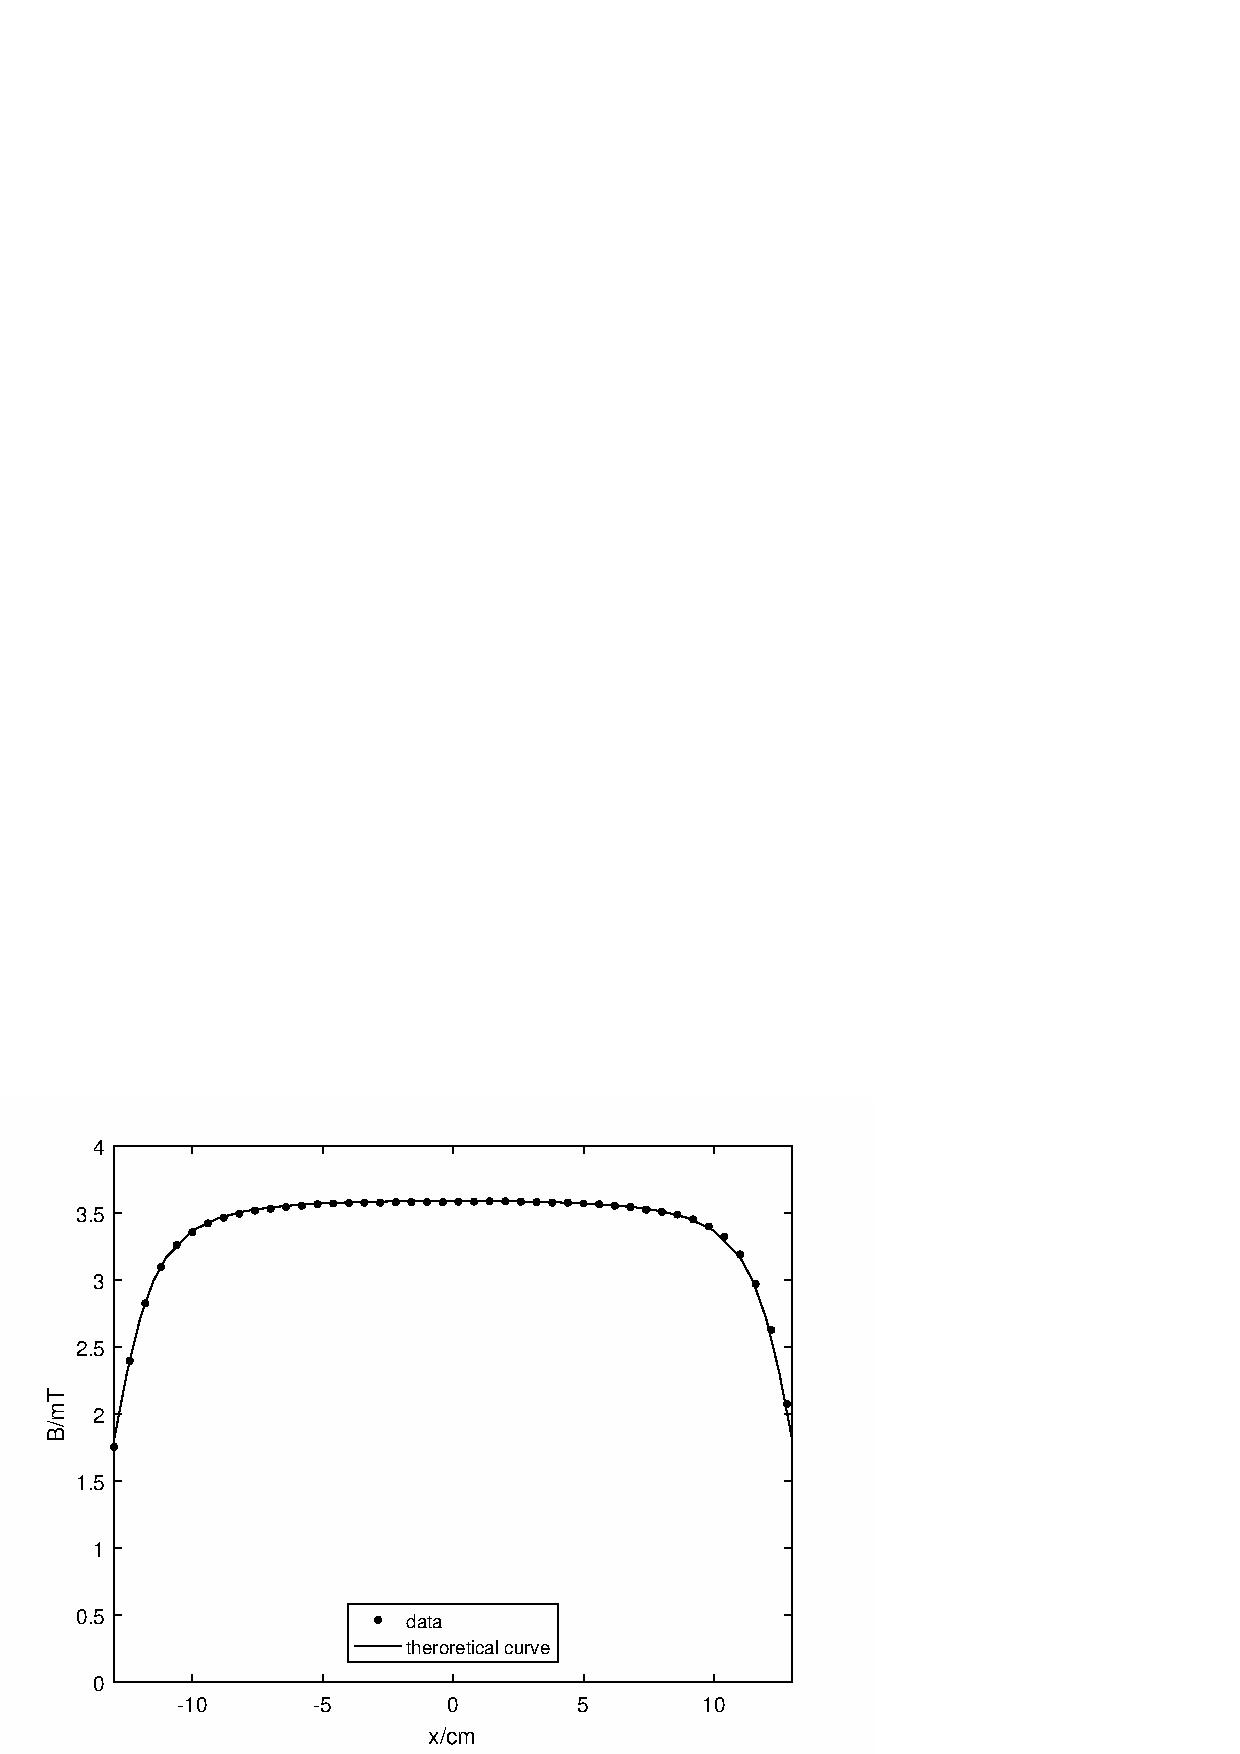
\includegraphics[scale=0.4]{fig3.png}
	\caption{Solar cell equivalent circuit.}
\end{figure}


\section{Measurement Setup and Procedure}

\subsection{Measurement Setup}
The setup consists of a photovoltaic device (5 W), a 300 W tungsten{halogen lamp
serving as a radiation source, two digital multimeters, two adjustable resistors, a solar power meter, a wiring board and a measuring tape.

\subsection{Measurement Procedure and Data Presentation}

\begin{enumerate}
\item
Turn on both the light and the fan. Wait for at least five minutes, in order to let
the light reach its working intensity.
\item
Design a measuring circuit with the photovoltaic device, multimeters set in an appropriate range, and the resistance. Connect the elements into a circuit using the
provided wiring board.
\item
Change the resistance, measure the relevant current and voltage to draw the I-V
characteristics curve. Keep the distance between the light source and the photo-
voltaic device and do not move around the workstation during the measurement, to
ensure the same light intensity is maintained during the whole process.
\item
Measure the I-V characteristics curves and the values of $V_{oc}$ and $I_{sc}$ under each of the following conditions:
\begin{enumerate}[(a)]
\item
The distance between the light source and the photovoltaic device is 100 cm;
Measure the solar power by the provided solar power meter.
\item
The distance between the light source and the photovoltaic device is 120 cm;
Measure the solar power by the provided solar power meter.
\item
The distance between the light source and the photovoltaic device is 120 cm,
with two devices in series.
\item
The distance between the light source and the photovoltaic device is 120 cm,
with two devices in parallel.
\end{enumerate}
\item
Plot (use a computer)
\begin{enumerate}[(a)]
\item
the I-V characteristics curves;
\item
the graph of the output power vs. the voltage. Determine the values of
$I_{sc}$, $V_{oc}$, $P_m$, $I_m$, $V_m$, $R_m$, $FF$, and $\eta$. Compile the data in the form of a table.
\end{enumerate}
\end{enumerate}


\section{Results}

The multimeter precision was shown in Table \ref{tab-1}.

\begin{table}[!h]
\begin{center}
\begin{tabular}{|c|c|}
\hline
QUANTITY & PRECISION \\
\hline
DC voltage & $0.5\%+\Delta$ [V]\\
\hline
DC current & $1.5\%+\Delta$ [mA]\\
\hline
distance & $0.1$ [cm]\\
\hline
solar power & $10$ [$\rm W/m^2$]\\
\hline
\end{tabular}
\caption{Multimeter precision.}
\label{tab-1}
\end{center}
\end{table}

The measurement data for area was shown in Table \ref{tab-2}.

\begin{table}[!h]
\begin{center}
\begin{tabular}{|c|c|}
\hline
length [cm] & width [cm] \\
\hline
21.0 & 26.0 \\
\hline
\end{tabular}
\caption{Measurement data for area.}
\label{tab-2}
\end{center}
\end{table}

$$S=21\times26=546.0\pm3.3\,\rm cm^2$$

The measurement data for solar power was shown in Table \ref{tab-3}.

\begin{table}[!h]
\begin{center}
\begin{tabular}{|c|c|c|c|c|c|}
\hline
& 0 & 1 & 2 & 3 & 4 \\
\hline
$P_{100}$ [$\rm W/m^2$] & 270 & 324 & 439 & 499 & 532 \\
\hline
$P_{120}$ [$\rm W/m^2$] & 203 & 257 & 334 & 381 & 406 \\
\hline
\end{tabular}
\caption{Measurement data for solar power.}
\label{tab-3}
\end{center}
\end{table}

$$P_{100}=\frac{270+324+439+499+532}{5}=412.6\pm10.0 \,\rm W/m^2$$
$$P_{in}=22.52\pm0.56\,\rm W$$
$$P_{120}=\frac{203+257+334+381+406}{5}=316.2\pm10.0 \,\rm W/m^2$$
$$P_{in}=17.26\pm0.56\,\rm W$$


The measurement data for $U_{oc}$ and $I_{sc}$ was shown in Table \ref{tab-4}.

\begin{table}[!h]
\begin{center}
\begin{tabular}{|c|c|c|c|c|}
\hline
& 100 cm & 120 cm & series & parallel \\
\hline
$U_{oc}$ [V] & 9.98 & 9.66 & 19.10 & 9.55\\
\hline
$I_{sc}$ [mA] & 105.2 & 84.4 & 92.3 & 184.0 \\
\hline
\end{tabular}
\caption{Measurement data for $U_{oc}$ and $I_{sc}$.}
\label{tab-4}
\end{center}
\end{table}

\newpage

The measurement of a solar cell was shown in Table \ref{tab-5}.\\

\begin{table}[!h]
\begin{center}
\begin{tabular}{|c|c|c|c|c|}
\hline
&\multicolumn{2}{|c|}{100 cm}&\multicolumn{2}{|c|}{120 cm}\\
\hline
& $U$ [V] & $I$ [mA] & $U$ [V] & $I$ [mA] \\
\hline
1	&	0.18	&	104.7	&	0.34	&	89.9	\\
\hline
2	&	0.92	&	102.7	&	1.06	&	88.1	\\
\hline
3	&	1.78	&	99.8	&	1.93	&	85.7	\\
\hline
4	&	2.32	&	97.9	&	2.72	&	83.9	\\
\hline
5	&	2.81	&	95.7	&	3.09	&	83.0	\\
\hline
6	&	3.21	&	94.1	&	3.63	&	81.7	\\
\hline
7	&	3.76	&	91.9	&	4.29	&	79.5	\\
\hline
8	&	4.47	&	89.6	&	4.76	&	77.6	\\
\hline
9	&	4.94	&	88.5	&	5.29	&	76.2	\\
\hline
10	&	5.95	&	84.2	&	5.85	&	74.0	\\
\hline
11	&	6.65	&	81.3	&	6.24	&	72.2	\\
\hline
12	&	7.30	&	78.4	&	6.43	&	70.3	\\
\hline
13	&	7.69	&	76.5	&	6.61	&	68.5	\\
\hline
14	&	7.69	&	76.5	&	7.11	&	67.2	\\
\hline
15	&	7.85	&	75.4	&	7.60	&	63.9	\\
\hline
16	&	8.04	&	74.1	&	8.07	&	59.5	\\
\hline
17	&	8.26	&	72.2	&	8.33	&	55.6	\\
\hline
18	&	8.52	&	70.7	&	8.52	&	51.9	\\
\hline
19	&	8.70	&	65.9	&	8.66	&	48.5	\\
\hline
20	&	8.78	&	63.8	&	8.78	&	45.3	\\
\hline
21	&	8.89	&	61.0	&	8.91	&	41.4	\\
\hline
22	&	9.34	&	44.3	&	9.03	&	37.1	\\
\hline
23	&	9.66	&	26.7	&	9.27	&	27.6	\\
\hline
24	&	9.82	&	15.2	&	9.52	&	14.9	\\
\hline
25	&	9.92	&	8.5	&	9.62	&	8.2	\\
\hline
\end{tabular}
\caption{Measurement Data for the $U$ vs. $I$ relation (100 cm/120 cm configuration).}
\label{tab-5}
\end{center}
\end{table}

\newpage

The measurement of two solar cells was shown in Table \ref{tab-6}.\\

\begin{table}[!h]
\begin{center}
\begin{tabular}{|c|c|c|c|c|}
\hline
&\multicolumn{2}{|c|}{100 cm}&\multicolumn{2}{|c|}{120 cm}\\
\hline
& $U$ [V] & $I$ [mA] & $U$ [V] & $I$ [mA] \\
\hline
1	&	0.22	&	92.3	&	0.11	&	184.5	\\
\hline
2	&	1.23	&	91.3	&	0.69	&	180.8	\\
\hline
3	&	2.21	&	90.1	&	1.28	&	177.8	\\
\hline
4	&	3.23	&	88.5	&	1.72	&	175.2	\\
\hline
5	&	4.21	&	87.2	&	2.27	&	172.0	\\
\hline
6	&	5.20	&	85.8	&	2.83	&	169.2	\\
\hline
7	&	6.25	&	84.1	&	3.33	&	166.2	\\
\hline
8	&	7.29	&	82.7	&	3.82	&	162.6	\\
\hline
9	&	8.10	&	80.9	&	4.38	&	159.0	\\
\hline
10	&	8.43	&	80.4	&	4.61	&	157.4	\\
\hline
11	&	9.01	&	78.8	&	4.83	&	156.2	\\
\hline
12	&	9.40	&	78.2	&	5.03	&	154.5	\\
\hline
13	&	10.03	&	77.0	&	5.26	&	152.7	\\
\hline
14	&	10.85	&	75.6	&	5.44	&	150.7	\\
\hline
15	&	11.60	&	73.7	&	5.64	&	148.5	\\
\hline
16	&	12.43	&	70.9	&	5.99	&	143.6	\\
\hline
17	&	13.30	&	67.3	&	6.43	&	136.4	\\
\hline
18	&	14.04	&	64.6	&	6.83	&	128.6	\\
\hline
19	&	14.86	&	60.3	&	7.22	&	119.9	\\
\hline
20	&	15.71	&	53.4	&	7.67	&	108.2	\\
\hline
21	&	16.54	&	44.9	&	8.05	&	95.5	\\
\hline
22	&	17.45	&	32.6	&	8.43	&	79.5	\\
\hline
23	&	17.96	&	24.0	&	8.93	&	50.8	\\
\hline
24	&	18.20	&	20.1	&	9.34	&	20.0	\\
\hline
25	&	18.41	&	16.2	&	9.46	&	8.2	\\
\hline
\end{tabular}
\caption{Measurement Data for the $U$ vs. $I$ relation (series/parallel configuration).}
\label{tab-6}
\end{center}
\end{table}

\newpage

For the first 100 cm circuit,\\

The compiled data was shown in Table \ref{tab-com-1}.\\

\begin{table}[!h]
\begin{center}
\begin{tabular}{|c|c|c|c|c|}
\hline
& $U$ [V] & $I$ [mA] & $P$ [mW] & $R$ [$\rm \Omega$] \\
\hline
1	&	$0.18 \pm 0.01$	&	$104.7 \pm 1.7$	&	$18.85 \pm 1.18$	&	$1.72 \pm 0.11$	\\
\hline
2	&	$0.92 \pm 0.01$	&	$102.7 \pm 1.6$	&	$94.48 \pm 2.13$	&	$8.96 \pm 0.20$	\\
\hline
3	&	$1.78 \pm 0.02$	&	$99.8 \pm 1.6$	&	$177.64 \pm 3.41$	&	$17.84 \pm 0.34$	\\
\hline
4	&	$2.32 \pm 0.02$	&	$97.9 \pm 1.6$	&	$227.13 \pm 4.21$	&	$23.70 \pm 0.44$	\\
\hline
5	&	$2.81 \pm 0.02$	&	$95.7 \pm 1.5$	&	$268.92 \pm 4.89$	&	$29.36 \pm 0.53$	\\
\hline
6	&	$3.21 \pm 0.03$	&	$94.1 \pm 1.5$	&	$302.06 \pm 5.44$	&	$34.11 \pm 0.61$	\\
\hline
7	&	$3.76 \pm 0.03$	&	$91.9 \pm 1.5$	&	$345.54 \pm 6.16$	&	$40.91 \pm 0.73$	\\
\hline
8	&	$4.47 \pm 0.03$	&	$89.6 \pm 1.4$	&	$400.51 \pm 7.08$	&	$49.89 \pm 0.88$	\\
\hline
9	&	$4.94 \pm 0.03$	&	$88.5 \pm 1.4$	&	$437.19 \pm 7.69$	&	$55.82 \pm 0.98$	\\
\hline
10	&	$5.95 \pm 0.04$	&	$84.2 \pm 1.4$	&	$500.99 \pm 8.77$	&	$70.67 \pm 1.24$	\\
\hline
11	&	$6.65 \pm 0.04$	&	$81.3 \pm 1.3$	&	$540.64 \pm 9.45$	&	$81.80 \pm 1.43$	\\
\hline
12	&	$7.30 \pm 0.05$	&	$78.4 \pm 1.3$	&	$572.32 \pm 10.00$	&	$93.11 \pm 1.63$	\\
\hline
13	&	$7.69 \pm 0.05$	&	$76.5 \pm 1.2$	&	$588.29 \pm 10.28$	&	$100.52 \pm 1.76$	\\
\hline
14	&	$7.69 \pm 0.05$	&	$76.5 \pm 1.2$	&	$588.29 \pm 10.28$	&	$100.52 \pm 1.76$	\\
\hline
15	&	$7.85 \pm 0.05$	&	$75.4 \pm 1.2$	&	$591.89 \pm 10.35$	&	$104.11 \pm 1.82$	\\
\hline
16	&	$8.04 \pm 0.05$	&	$74.1 \pm 1.2$	&	$595.76 \pm 10.43$	&	$108.50 \pm 1.90$	\\
\hline
17	&	$8.26 \pm 0.05$	&	$72.2 \pm 1.2$	&	$596.37 \pm 10.45$	&	$114.40 \pm 2.00$	\\
\hline
18	&	$8.52 \pm 0.05$	&	$70.7 \pm 1.2$	&	$602.36 \pm 10.56$	&	$120.51 \pm 2.11$	\\
\hline
19	&	$8.70 \pm 0.05$	&	$65.9 \pm 1.1$	&	$573.33 \pm 10.10$	&	$132.02 \pm 2.33$	\\
\hline
20	&	$8.78 \pm 0.05$	&	$63.8 \pm 1.1$	&	$560.16 \pm 9.90$	&	$137.62 \pm 2.43$	\\
\hline
21	&	$8.89 \pm 0.05$	&	$61.0 \pm 1.0$	&	$542.29 \pm 9.62$	&	$145.74 \pm 2.58$	\\
\hline
22	&	$9.34 \pm 0.06$	&	$44.3 \pm 0.8$	&	$413.76 \pm 7.57$	&	$210.84 \pm 3.86$	\\
\hline
23	&	$9.66 \pm 0.06$	&	$26.7 \pm 0.5$	&	$257.92 \pm 5.08$	&	$361.80 \pm 7.12$	\\
\hline
24	&	$9.82 \pm 0.06$	&	$15.2 \pm 0.3$	&	$149.26 \pm 3.34$	&	$646.05 \pm 14.47$	\\
\hline
25	&	$9.92 \pm 0.06$	&	$8.5 \pm 0.2$	&	$84.32 \pm 2.31$	&	$1167.06 \pm 32.01$	\\
\hline
\end{tabular}
\caption{Compiled data for the first 100 cm circuit.}
\label{tab-com-1}
\end{center}
\end{table}

$$I_{sc}=105.2\pm1.7\,{\rm mA},\quad U_{oc}=9.98\pm0.06\,{\rm V}$$
$$P_m=602.36\pm10.56\,{\rm mW},\quad I_m=70.7\pm1.2\,{\rm mA},\quad U_m=8.52\pm0.05\,{\rm V}$$
$$R_m=\frac{U_m}{I_m}=120.51\pm2.11\,{\rm \Omega}$$
$$FF=\frac{P_m}{U_{oc}I_{sc}}=0.574\pm0.014$$
$$\eta=\frac{P_m}{P_{in}}=2.67\pm0.08\,\%$$
$$$$

The $I-V$ characteristics curve is plotted in Figure \ref{IV-1}.
\begin{figure}[H]
\centering
\includegraphics[scale=0.6]{IV1.png}
\caption{The $I-V$ characteristics curve.}
\label{IV-1}
\end{figure}
The graph of the output power vs. the vlotage is plotted in Figure \ref{PV-1}.
\begin{figure}[H]
\centering
\includegraphics[scale=0.6]{PV1.png}
\caption{The graph of the output power vs. the voltage.}
\label{PV-1}
\end{figure}
The graph of the output power vs. the resistance is plotted in Figure \ref{PR-1}.
\begin{figure}[H]
\centering
\includegraphics[scale=0.6]{PR1.png}
\caption{The graph of the output power vs. the resistance.}
\label{PR-1}
\end{figure}
$$$$

For the second 120 cm circuit,\\

The compiled data was shown in Table \ref{tab-com-2}.\\

\begin{table}[!h]
\begin{center}
\begin{tabular}{|c|c|c|c|c|}
\hline
& $U$ [V] & $I$ [mA] & $P$ [mW] & $R$ [$\rm \Omega$] \\
\hline
1	&	$0.34 \pm 0.01$	&	$89.9 \pm 1.4$	&	$30.57 \pm 1.16$	&	$3.78 \pm 0.14$	\\
\hline
2	&	$1.06 \pm 0.02$	&	$88.1 \pm 1.4$	&	$93.39 \pm 2.02$	&	$12.03 \pm 0.26$	\\
\hline
3	&	$1.93 \pm 0.02$	&	$85.7 \pm 1.4$	&	$165.40 \pm 3.16$	&	$22.52 \pm 0.43$	\\
\hline
4	&	$2.72 \pm 0.02$	&	$83.9 \pm 1.4$	&	$228.21 \pm 4.19$	&	$32.42 \pm 0.60$	\\
\hline
5	&	$3.09 \pm 0.03$	&	$83.0 \pm 1.3$	&	$256.47 \pm 4.66$	&	$37.23 \pm 0.68$	\\
\hline
6	&	$3.63 \pm 0.03$	&	$81.7 \pm 1.3$	&	$296.57 \pm 5.33$	&	$44.43 \pm 0.80$	\\
\hline
7	&	$4.29 \pm 0.03$	&	$79.5 \pm 1.3$	&	$341.06 \pm 6.08$	&	$53.96 \pm 0.96$	\\
\hline
8	&	$4.76 \pm 0.03$	&	$77.6 \pm 1.3$	&	$369.38 \pm 6.56$	&	$61.34 \pm 1.09$	\\
\hline
9	&	$5.29 \pm 0.04$	&	$76.2 \pm 1.2$	&	$403.10 \pm 7.14$	&	$69.42 \pm 1.23$	\\
\hline
10	&	$5.85 \pm 0.04$	&	$74.0 \pm 1.2$	&	$432.90 \pm 7.65$	&	$79.05 \pm 1.40$	\\
\hline
11	&	$6.24 \pm 0.04$	&	$72.2 \pm 1.2$	&	$450.53 \pm 7.96$	&	$86.43 \pm 1.53$	\\
\hline
12	&	$6.43 \pm 0.04$	&	$70.3 \pm 1.2$	&	$452.03 \pm 7.99$	&	$91.47 \pm 1.62$	\\
\hline
13	&	$6.61 \pm 0.04$	&	$68.5 \pm 1.1$	&	$452.79 \pm 8.01$	&	$96.50 \pm 1.71$	\\
\hline
14	&	$7.11 \pm 0.05$	&	$67.2 \pm 1.1$	&	$477.79 \pm 8.45$	&	$105.80 \pm 1.87$	\\
\hline
15	&	$7.60 \pm 0.05$	&	$63.9 \pm 1.1$	&	$485.64 \pm 8.61$	&	$118.94 \pm 2.11$	\\
\hline
16	&	$8.07 \pm 0.05$	&	$59.5 \pm 1.0$	&	$480.17 \pm 8.55$	&	$135.63 \pm 2.42$	\\
\hline
17	&	$8.33 \pm 0.05$	&	$55.6 \pm 0.9$	&	$463.15 \pm 8.29$	&	$149.82 \pm 2.68$	\\
\hline
18	&	$8.52 \pm 0.05$	&	$51.9 \pm 0.9$	&	$442.19 \pm 7.97$	&	$164.16 \pm 2.96$	\\
\hline
19	&	$8.66 \pm 0.05$	&	$48.5 \pm 0.8$	&	$420.01 \pm 7.62$	&	$178.56 \pm 3.24$	\\
\hline
20	&	$8.78 \pm 0.05$	&	$45.3 \pm 0.8$	&	$397.73 \pm 7.27$	&	$193.82 \pm 3.54$	\\
\hline
21	&	$8.91 \pm 0.05$	&	$41.4 \pm 0.7$	&	$368.87 \pm 6.81$	&	$215.22 \pm 3.97$	\\
\hline
22	&	$9.03 \pm 0.06$	&	$37.1 \pm 0.7$	&	$335.01 \pm 6.27$	&	$243.40 \pm 4.56$	\\
\hline
23	&	$9.27 \pm 0.06$	&	$27.6 \pm 0.5$	&	$255.85 \pm 5.01$	&	$335.87 \pm 6.58$	\\
\hline
24	&	$9.52 \pm 0.06$	&	$14.9 \pm 0.3$	&	$141.85 \pm 3.20$	&	$638.93 \pm 14.40$	\\
\hline
25	&	$9.62 \pm 0.06$	&	$8.2 \pm 0.2$	&	$78.88 \pm 2.20$	&	$1173.17 \pm 32.68$	\\
\hline
\end{tabular}
\caption{Compiled data for the second 120 cm circuit.}
\label{tab-com-2}
\end{center}
\end{table}

$$I_{sc}=84.4\pm1.4\,{\rm mA},\quad U_{oc}=9.66\pm0.06\,{\rm V}$$
$$P_m=485.64\pm8.61\,{\rm mW},\quad I_m=63.9\pm1.1\,{\rm mA},\quad U_m=7.60\pm0.05\,{\rm V}$$
$$R_m=\frac{U_m}{I_m}=118.94\pm2.11\,{\rm \Omega}$$
$$FF=\frac{P_m}{U_{oc}I_{sc}}=0.596\pm0.015$$
$$\eta=\frac{P_m}{P_{in}}=2.81\pm0.10\,\%$$
$$$$

The $I-V$ characteristics curve is plotted in Figure \ref{IV-2}.
\begin{figure}[H]
\centering
\includegraphics[scale=0.6]{IV2.png}
\caption{The $I-V$ characteristics curve.}
\label{IV-2}
\end{figure}
The graph of the output power vs. the vlotage is plotted in Figure \ref{PV-2}.
\begin{figure}[H]
\centering
\includegraphics[scale=0.6]{PV2.png}
\caption{The graph of the output power vs. the voltage.}
\label{PV-2}
\end{figure}
The graph of the output power vs. the resistance is plotted in Figure \ref{PR-2}.
\begin{figure}[H]
\centering
\includegraphics[scale=0.6]{PR2.png}
\caption{The graph of the output power vs. the resistance.}
\label{PR-2}
\end{figure}
$$$$

For the third series circuit,\\

The compiled data was shown in Table \ref{tab-com-3}.\\

\begin{table}[!h]
\begin{center}
\begin{tabular}{|c|c|c|c|c|}
\hline
& $U$ [V] & $I$ [mA] & $P$ [mW] & $R$ [$\rm \Omega$] \\
\hline
1	&	$0.22 \pm 0.01$	&	$92.3 \pm 1.5$	&	$20.31 \pm 1.08$	&	$2.38 \pm 0.13$	\\
\hline
2	&	$1.23 \pm 0.02$	&	$91.3 \pm 1.5$	&	$112.30 \pm 2.33$	&	$13.47 \pm 0.28$	\\
\hline
3	&	$2.21 \pm 0.02$	&	$90.1 \pm 1.5$	&	$199.12 \pm 3.73$	&	$24.53 \pm 0.46$	\\
\hline
4	&	$3.23 \pm 0.03$	&	$88.5 \pm 1.4$	&	$285.86 \pm 5.16$	&	$36.50 \pm 0.66$	\\
\hline
5	&	$4.21 \pm 0.03$	&	$87.2 \pm 1.4$	&	$367.11 \pm 6.52$	&	$48.28 \pm 0.86$	\\
\hline
6	&	$5.20 \pm 0.04$	&	$85.8 \pm 1.4$	&	$446.16 \pm 7.85$	&	$60.61 \pm 1.07$	\\
\hline
7	&	$6.25 \pm 0.04$	&	$84.1 \pm 1.4$	&	$525.63 \pm 9.19$	&	$74.32 \pm 1.30$	\\
\hline
8	&	$7.29 \pm 0.05$	&	$82.7 \pm 1.3$	&	$602.88 \pm 10.50$	&	$88.15 \pm 1.54$	\\
\hline
9	&	$8.10 \pm 0.05$	&	$80.9 \pm 1.3$	&	$655.29 \pm 11.40$	&	$100.12 \pm 1.74$	\\
\hline
10	&	$8.43 \pm 0.05$	&	$80.4 \pm 1.3$	&	$677.77 \pm 11.78$	&	$104.85 \pm 1.82$	\\
\hline
11	&	$9.01 \pm 0.06$	&	$78.8 \pm 1.3$	&	$709.99 \pm 12.34$	&	$114.34 \pm 1.99$	\\
\hline
12	&	$9.40 \pm 0.06$	&	$78.2 \pm 1.3$	&	$735.08 \pm 12.77$	&	$120.20 \pm 2.09$	\\
\hline
13	&	$10.03 \pm 0.06$	&	$77.0 \pm 1.3$	&	$772.31 \pm 13.41$	&	$130.26 \pm 2.26$	\\
\hline
14	&	$10.85 \pm 0.06$	&	$75.6 \pm 1.2$	&	$820.26 \pm 14.24$	&	$143.52 \pm 2.49$	\\
\hline
15	&	$11.60 \pm 0.07$	&	$73.7 \pm 1.2$	&	$854.92 \pm 14.85$	&	$157.39 \pm 2.73$	\\
\hline
16	&	$12.43 \pm 0.07$	&	$70.9 \pm 1.2$	&	$881.29 \pm 15.34$	&	$175.32 \pm 3.05$	\\
\hline
17	&	$13.30 \pm 0.08$	&	$67.3 \pm 1.1$	&	$895.09 \pm 15.63$	&	$197.62 \pm 3.45$	\\
\hline
18	&	$14.04 \pm 0.08$	&	$64.6 \pm 1.1$	&	$906.98 \pm 15.88$	&	$217.34 \pm 3.80$	\\
\hline
19	&	$14.86 \pm 0.08$	&	$60.3 \pm 1.0$	&	$896.06 \pm 15.77$	&	$246.43 \pm 4.34$	\\
\hline
20	&	$15.71 \pm 0.09$	&	$53.4 \pm 0.9$	&	$838.91 \pm 14.92$	&	$294.19 \pm 5.23$	\\
\hline
21	&	$16.54 \pm 0.09$	&	$44.9 \pm 0.8$	&	$742.65 \pm 13.45$	&	$368.37 \pm 6.67$	\\
\hline
22	&	$17.45 \pm 0.10$	&	$32.6 \pm 0.6$	&	$568.87 \pm 10.76$	&	$535.28 \pm 10.12$	\\
\hline
23	&	$17.96 \pm 0.10$	&	$24.0 \pm 0.5$	&	$431.04 \pm 8.60$	&	$748.33 \pm 14.93$	\\
\hline
24	&	$18.20 \pm 0.10$	&	$20.1 \pm 0.4$	&	$365.82 \pm 7.58$	&	$905.47 \pm 18.77$	\\
\hline
25	&	$18.41 \pm 0.10$	&	$16.2 \pm 0.3$	&	$298.24 \pm 6.53$	&	$1136.42 \pm 24.87$	\\
\hline
\end{tabular}
\caption{Compiled data for the third series circuit.}
\label{tab-com-3}
\end{center}
\end{table}

$$I_{sc}=82.3\pm1.3\,{\rm mA},\quad U_{oc}=19.10\pm0.11\,{\rm V}$$
$$P_m=906.98\pm15.88\,{\rm mW},\quad I_m=64.6\pm1.1\,{\rm mA},\quad U_m=14.04\pm0.08\,{\rm V}$$
$$R_m=\frac{U_m}{I_m}=217.34\pm3.80\,{\rm \Omega}$$
$$FF=\frac{P_m}{U_{oc}I_{sc}}=0.577\pm0.014$$
$$\eta=\frac{P_m}{P_{in}}=2.01\pm0.06\,\%$$
$$$$

The $I-V$ characteristics curve is plotted in Figure \ref{IV-3}.
\begin{figure}[H]
\centering
\includegraphics[scale=0.6]{IV3.png}
\caption{The $I-V$ characteristics curve.}
\label{IV-3}
\end{figure}
The graph of the output power vs. the vlotage is plotted in Figure \ref{PV-3}.
\begin{figure}[H]
\centering
\includegraphics[scale=0.6]{PV3.png}
\caption{The graph of the output power vs. the voltage.}
\label{PV-3}
\end{figure}
The graph of the output power vs. the resistance is plotted in Figure \ref{PR-3}.
\begin{figure}[H]
\centering
\includegraphics[scale=0.6]{PR3.png}
\caption{The graph of the output power vs. the resistance.}
\label{PR-3}
\end{figure}
$$$$

For the fourth parallel circuit,\\

The compiled data was shown in Table \ref{tab-com-4}.\\

\begin{table}[!h]
\begin{center}
\begin{tabular}{|c|c|c|c|c|}
\hline
& $U$ [V] & $I$ [mA] & $P$ [mW] & $R$ [$\rm \Omega$] \\
\hline
1	&	$0.11 \pm 0.01$	&	$184.5 \pm 2.9$	&	$20.30 \pm 1.97$	&	$0.60 \pm 0.06$	\\
\hline
2	&	$0.69 \pm 0.01$	&	$180.8 \pm 2.8$	&	$124.75 \pm 3.11$	&	$3.82 \pm 0.10$	\\
\hline
3	&	$1.28 \pm 0.02$	&	$177.8 \pm 2.8$	&	$227.58 \pm 4.59$	&	$7.20 \pm 0.15$	\\
\hline
4	&	$1.72 \pm 0.02$	&	$175.2 \pm 2.7$	&	$301.34 \pm 5.71$	&	$9.82 \pm 0.19$	\\
\hline
5	&	$2.27 \pm 0.02$	&	$172.0 \pm 2.7$	&	$390.44 \pm 7.11$	&	$13.20 \pm 0.24$	\\
\hline
6	&	$2.83 \pm 0.02$	&	$169.2 \pm 2.6$	&	$478.84 \pm 8.51$	&	$16.73 \pm 0.30$	\\
\hline
7	&	$3.33 \pm 0.03$	&	$166.2 \pm 2.6$	&	$553.45 \pm 9.70$	&	$20.04 \pm 0.35$	\\
\hline
8	&	$3.82 \pm 0.03$	&	$162.6 \pm 2.5$	&	$621.13 \pm 10.79$	&	$23.49 \pm 0.41$	\\
\hline
9	&	$4.38 \pm 0.03$	&	$159.0 \pm 2.5$	&	$696.42 \pm 12.01$	&	$27.55 \pm 0.47$	\\
\hline
10	&	$4.61 \pm 0.03$	&	$157.4 \pm 2.5$	&	$725.61 \pm 12.48$	&	$29.29 \pm 0.50$	\\
\hline
11	&	$4.83 \pm 0.03$	&	$156.2 \pm 2.4$	&	$754.45 \pm 12.95$	&	$30.92 \pm 0.53$	\\
\hline
12	&	$5.03 \pm 0.04$	&	$154.5 \pm 2.4$	&	$777.13 \pm 13.32$	&	$32.56 \pm 0.56$	\\
\hline
13	&	$5.26 \pm 0.04$	&	$152.7 \pm 2.4$	&	$803.20 \pm 13.74$	&	$34.45 \pm 0.59$	\\
\hline
14	&	$5.44 \pm 0.04$	&	$150.7 \pm 2.4$	&	$819.81 \pm 14.01$	&	$36.10 \pm 0.62$	\\
\hline
15	&	$5.64 \pm 0.04$	&	$148.5 \pm 2.3$	&	$837.54 \pm 14.30$	&	$37.98 \pm 0.65$	\\
\hline
16	&	$5.99 \pm 0.04$	&	$143.6 \pm 2.3$	&	$860.16 \pm 14.67$	&	$41.71 \pm 0.71$	\\
\hline
17	&	$6.43 \pm 0.04$	&	$136.4 \pm 2.1$	&	$877.05 \pm 14.95$	&	$47.14 \pm 0.80$	\\
\hline
18	&	$6.83 \pm 0.04$	&	$128.6 \pm 2.0$	&	$878.34 \pm 14.98$	&	$53.11 \pm 0.91$	\\
\hline
19	&	$7.22 \pm 0.05$	&	$119.9 \pm 1.9$	&	$865.68 \pm 14.78$	&	$60.22 \pm 1.03$	\\
\hline
20	&	$7.67 \pm 0.05$	&	$108.2 \pm 1.7$	&	$829.89 \pm 14.21$	&	$70.89 \pm 1.21$	\\
\hline
21	&	$8.05 \pm 0.05$	&	$95.5 \pm 1.5$	&	$768.78 \pm 13.24$	&	$84.29 \pm 1.45$	\\
\hline
22	&	$8.43 \pm 0.05$	&	$79.5 \pm 1.3$	&	$670.18 \pm 11.66$	&	$106.04 \pm 1.84$	\\
\hline
23	&	$8.93 \pm 0.05$	&	$50.8 \pm 0.9$	&	$453.64 \pm 8.18$	&	$175.79 \pm 3.17$	\\
\hline
24	&	$9.34 \pm 0.06$	&	$20.0 \pm 0.4$	&	$186.80 \pm 3.90$	&	$467.00 \pm 9.76$	\\
\hline
25	&	$9.46 \pm 0.06$	&	$8.2 \pm 0.2$	&	$77.57 \pm 2.16$	&	$1153.66 \pm 32.14$	\\
\hline
\end{tabular}
\caption{Compiled data for the fourth parallel circuit.}
\label{tab-com-4}
\end{center}
\end{table}

$$I_{sc}=184.0\pm2.9\,{\rm mA},\quad U_{oc}=9.55\pm0.06\,{\rm V}$$
$$P_m=878.34\pm14.98\,{\rm mW},\quad I_m=128.6\pm2.0\,{\rm mA},\quad U_m=6.83\pm0.04\,{\rm V}$$
$$R_m=\frac{U_m}{I_m}=53.11\pm0.91\,{\rm \Omega}$$
$$FF=\frac{P_m}{U_{oc}I_{sc}}=0.500\pm0.012$$
$$\eta=\frac{P_m}{P_{in}}=2.54\pm0.09\,\%$$
$$$$

The $I-V$ characteristics curve is plotted in Figure \ref{IV-4}.
\begin{figure}[H]
\centering
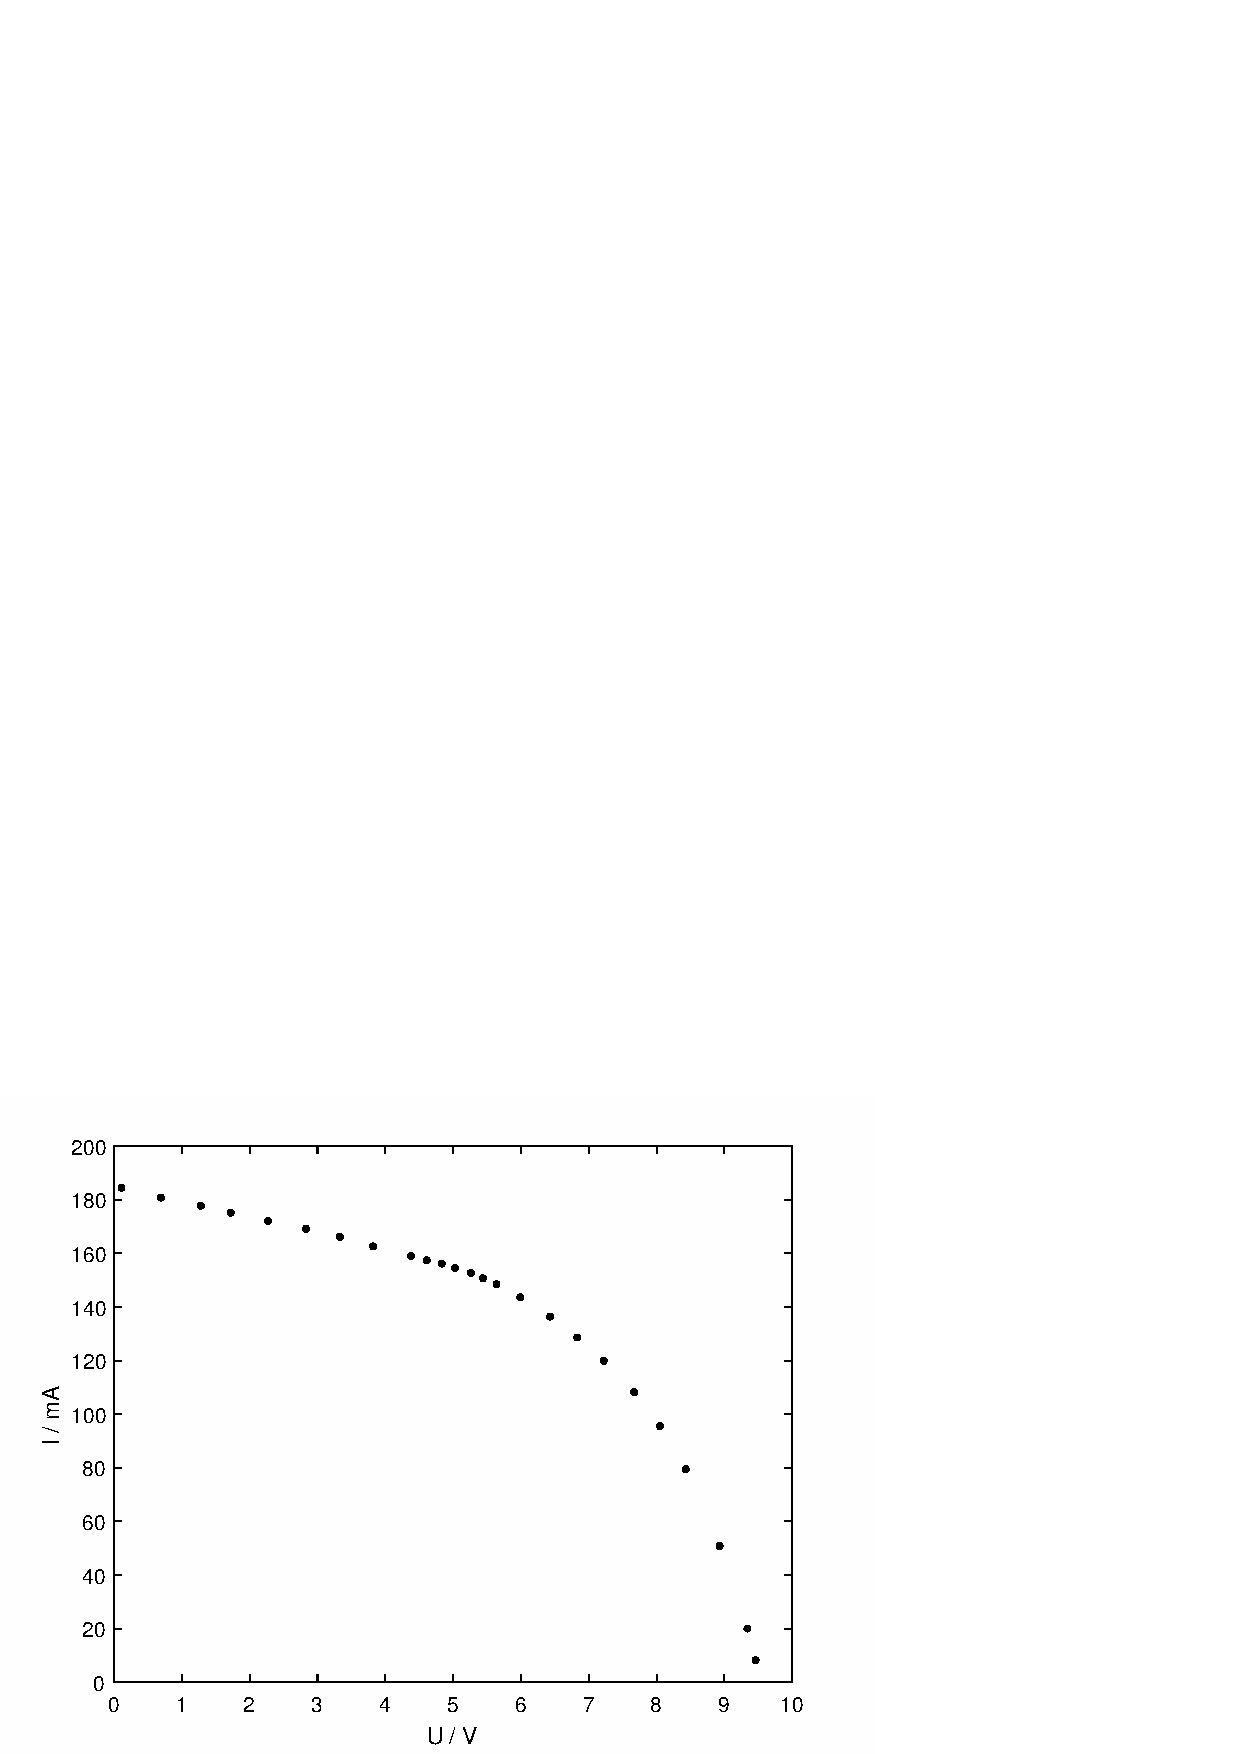
\includegraphics[scale=0.6]{IV4.png}
\caption{The $I-V$ characteristics curve.}
\label{IV-4}
\end{figure}
The graph of the output power vs. the vlotage is plotted in Figure \ref{PV-4}.
\begin{figure}[H]
\centering
\includegraphics[scale=0.6]{PV4.png}
\caption{The graph of the output power vs. the voltage.}
\label{PV-4}
\end{figure}
The graph of the output power vs. the resistance is plotted in Figure \ref{PR-4}.
\begin{figure}[H]
\centering
\includegraphics[scale=0.6]{PR4.png}
\caption{The graph of the output power vs. the resistance.}
\label{PR-4}
\end{figure}
$$$$



\newpage

\section{Measurement uncertainty analysis}

$S$ can be calculated by the equation $S=ab$. Therefore its uncertainty $u_S$ is found by applying the uncertainty propagation formula

\begin{align*}
u_S&=\sqrt{\left(\frac{\partial S}{\partial a}\right)^2u_a^2+\left(\frac{\partial S}{\partial b}\right)^2u_{b}^2}\\
&=\sqrt{b^2u_a^2+a^2u_b^2}\\
&=3.3\,\rm cm^2
\end{align*}

$$S=546.0\pm3.3\,\rm cm^2$$

$P_{in}$ can be calculated by the equation $P_{in}=P_xS$. Therefore its uncertainty $u_P$ is found by applying the uncertainty propagation formula

\begin{align*}
u_P&=\sqrt{\left(\frac{\partial P}{\partial P_x}\right)^2u_{P_x}^2+\left(\frac{\partial P}{\partial S}\right)^2u_{S}^2}\\
&=\sqrt{S^2u_{P_x}^2+P_x^2u_S^2}
\end{align*}

$$u_{P_{100}}=0.56\,\rm W$$
$$u_{P_{120}}=0.56\,\rm W$$

According to Table \ref{tab-1},

$$u_I=1.5\%I+0.1\,\rm mA$$
$$u_U=0.5\%U+0.01\,\rm V$$

$P$ can be calculated by the equation $P=UI$. Therefore its uncertainty $u_P$ is found by applying the uncertainty propagation formula

\begin{align*}
u_P&=\sqrt{\left(\frac{\partial P}{\partial U}\right)^2u_U^2+\left(\frac{\partial P}{\partial I}\right)^2u_{I}^2}\\
&=\sqrt{I^2u_U^2+U^2u_I^2}
\end{align*}

$R$ can be calculated by the equation $R=\frac{U}{I}$. Therefore its uncertainty $u_R$ is found by applying the uncertainty propagation formula

\begin{align*}
u_R&=\sqrt{\left(\frac{\partial R}{\partial U}\right)^2u_U^2+\left(\frac{\partial R}{\partial I}\right)^2u_{I}^2}\\
&=\sqrt{\left(\frac{1}{I}\right)^2u_U^2+\left(\frac{U}{I^2}\right)^2u_I^2}
\end{align*}

$FF$ can be calculated by the equation $FF=\frac{P_m}{P_{c}}$. Therefore its uncertainty $u_{FF}$ is found by applying the uncertainty propagation formula

\begin{align*}
u_{FF}&=\sqrt{\left(\frac{\partial FF}{\partial P_m}\right)^2u_{P_m}^2+\left(\frac{\partial FF}{\partial P_{c}}\right)^2u_{P_{c}}^2}\\
&=\sqrt{\left(\frac{1}{P_{c}}\right)^2u_{P_m}^2+\left(\frac{P_m}{{P_{c}}^2}\right)^2u_{P_{c}}^2}
\end{align*}

$\eta$ can be calculated by the equation $\eta=\frac{P_m}{P_{in}}$. Therefore its uncertainty $u_\eta$ is found by applying the uncertainty propagation formula

\begin{align*}
u_\eta&=\sqrt{\left(\frac{\partial \eta}{\partial P_m}\right)^2u_{P_m}^2+\left(\frac{\partial \eta}{\partial P_{in}}\right)^2u_{P_{in}}^2}\\
&=\sqrt{\left(\frac{1}{P_{in}}\right)^2u_{P_m}^2+\left(\frac{P_m}{{P_{in}}^2}\right)^2u_{P_{in}}^2}
\end{align*}

\section{Conclusion}

In this experiment, we measured the power supplied by the source and the power absorbed by the solar cells.\\

We found some properties of the solar cell by determine the values of
$I_{sc}$, $V_{oc}$, $P_m$, $I_m$, $V_m$, $R_m$, $FF$, and $\eta$.\\

We also plotted the I-V characteristics curve and the relation between power, voltage and resistance of the solar cell.\\

We use series and parallel method to connect two solar cells together and find that in a series circuit, the voltage superposed and in a parallel circuit the current superposed.\\

According the the value of $\eta$, we found that the efficiency of solar cell is very low.

\section{Reference}

\begin{enumerate}[(a)]
	\item
	Qin Tian, Han Xugen, Zheng Huan, Mateusz Krzyzosiak, VP241 Exercise 3, Solar Cells: I-V Characteristics, based on materials provided by the Department of Physics, Shanghai Jiaotong University.
\end{enumerate}

\section{Data sheet}

The Data sheet is attached at the end of the report.

\end{document}
